\documentclass[12pt, twoside, hidelinks, a4paper]{article}

\usepackage[]{geometry}
\geometry{inner=30mm, outer=20mm, top=23mm, bottom=23mm}

\usepackage{mystyle}
\pagestyle{headings}

\usepackage{fancyhdr}
\fancyhf{}
\pagestyle{fancy}
\renewcommand{\headrulewidth}{0pt}
% numery stron: lewa do lewego, prawa do prawego
\fancyfoot[LE,RO]{\thepage}

\fancypagestyle{plain}
{
   \fancyhf{}
\renewcommand{\headrulewidth}{0pt}
% numery stron: lewa do lewego, prawa do prawego
\fancyfoot[LE,RO]{\thepage}
}

\usepackage{pdfpages}
\usepackage{amsfonts}
%\renewcommand{\familydefault}{\sfdefault}
\setlength\parindent{1cm}

\usepackage{indentfirst}
\usepackage[affil-it]{authblk}
\usepackage{smartdiagram}
\usepackage{metalogo}
\usepackage{moreverb}

\let\lll\undefined
\usepackage{amssymb}

\begin{document}
    \setstretch{1.15}
 	\pagenumbering{arabic}

\author{Marcin Waszak}
\title{OWD -- sprawozdanie z projektu}
\date{5 grudnia 2018}
\affil{Wydział Elektroniki i Technik Informacyjnych, Politechnika Warszawska}


\maketitle

\begin{abstract}
Celem projektu jest optymalizacja pracy elektrowni pod względem kosztów jak i możliwości zaspokojenia wzrostu zapotrzebowań na energię ponad normę. Ponadto zostaną porównane techniki optymalizacji wielokryterialnej przy użyciu skalaryzacji \textit{Metodą Ważenia Ocen} (MWO) oraz \textit{Przedziałową Metodą Punktu Odniesienia} (PMPO).
\end{abstract}

\section{Zadanie}
Kod zadania: \textbf{OWD AK5}

Prowadzący projekt: dr inż. Adam Krzemienowski

\section{Analityczne sformułowanie problemu}
$P$ - uporządkowany zbiór okresów,

$T$ - uporządkowany zbiór typów generatorów (T1, T2, T3),

$I$ - uporządkowany zbiór generatorów danego typu,

Przyjmijmy: $p \in P$, $t \in T, i \in I[t]$

\subsection{Parametry}
\begin{itemize}
\item Zapotrzebowanie w danym okresie [MW]

$period\_demand \{P\}$
\item Długości okresów [h]

$period\_length \{P\}$
\item Ilość generatorów [szt]

$available\_generators \{T\}$
\item Obciążenie minimalne [MW]

$power\_min \{T\}$
\item Obciążenie maksymalne [MW]

$power\_max \{T\}$ 
\item Koszt przy min. obciążeniu [PLN/h]

$cost\_min \{T\}$ 
\item Koszt energii powyżej min. obciążenia [PLN/MWh]

$cost\_linear \{T\}$ 
\item Koszt uruchomienia [PLN]

$cost\_start \{T\}$
\item Całkowita wymagana energia w ciągu dnia [MWh]

$demand\_total = \sum_{p}^{p \in P} period\_demand[p] * period\_length[p]$
\end{itemize}

\subsection{Zmienne}
\begin{itemize}

%\item $\forall p \forall t \forall i : active{P,T,I} binary$
\item Flaga binarna informująca, czy zadany generator pracuje w danym okresie

$active\{P,T,I\} \; binary$
\item Moc danego generatora w danym okresie [MW]

$power\{P,T,I\}$
\item Faktyczna moc wszystkich generatorów w danym okresie

$period\_power \; \{p \in P\} = \sum_{t}^{t \in T} \sum_{i}^{i \in I[t]} \; power[p,t,i];$
\item Faktyczna wyprodukowana energia w ciągu dnia [MWh]

$production\_total = \sum_{p}^{p \in P} \; period\_power[p] * period\_length[p]$
\item 

$demand\_increase = \frac{production\_total}{demand\_total}$
\item Flaga zmiany stanu generatora wraz z początkiem danego okresu

(-1 = wyłączono, 0 = bez zmian, 1 = włączono)

$toggled \{p \in P, t \in T, i \in I[t] \} = active[p,t,i] - active[((p+3) mod |P|)+1,t,i]$

Warto wspomnieć, że dzięki użyciu modulo mamy ,,sklejony'' ostatni okres z pierwszym okresem. Z końcem dnia cykl zapotrzebowań się powtarza i ten fakt nasz model uwzględnia.
\item Flaga włączenia generatora z początkiem danego okresu

$started \{p \in P, t \in T, i \in I[t] \} = \frac{toggled[p,t,i]^2 + toggled[p,t,i]}{2}$
\item Koszt włączenia generatora w okresie (0 jeśli nie został włączony) [PLN]

$cost\_launch \{p \in P, t \in T, i \in I[t] \} = cost\_start[t] * started[p,t,i]$
\item Koszt pracy generatora po włączeniu [PLN/h]

$cost\_usage \{p \in P, t \in T, i \in I[t] \} = cost\_min[t] + cost\_linear[t] * (power[p,t,i] - power\_min[t])$
\item Dzienny całkowity koszt pracy elektrowni [PLN]

$cost\_total = \sum_{p}^{p \in P} \; \sum_{t}^{t \in T} \; \sum_{i}^{i \in I[t]} \; (period\_length[p] * cost\_usage[p,t,i] + cost\_launch[p,t,i])$
\end{itemize}


\subsection{Ograniczenia}
\begin{itemize}
%st1
\item Ograniczenie minimalnej mocy generatora. Zmienna binarna wyłącza te ograniczenie, kiedy dany generator nie pracuje

$\forall p \in P \; \forall t \in T \; \forall i \in I[t] \; : power[p,t,i] 
\geqslant power\_min[t] * active[p,t,i]$
%st2
\item Ograniczenie mocy maksymalnej generatora

$\forall p \in P \; \forall t \in T \; \forall i \in I[t] \; : power[p,t,i] \leqslant power\_max[t] * active[p,t,i]$
%st3
\item Każdemu włączonemu generatorowi T1 musi odpowiadać włączony generator T2 lub T3

$sum\_generators \{ p \in P, t \in T \} = \sum_{i}^{i \in I[t]} active[p,t,i]$

$\forall p \in P : sum\_generators[p,T1] \leqslant sum\_generators[p,T2] + sum\_generators[p,T3]$
%st4
\item Faktyczna dostarczana moc w ciągu okresu sprostać zapotrzebowaniom

$\forall p \in P : period_power[p] \geqslant period\_demand[p]$
\end{itemize}

\subsection{Funkcje celu}
\subsubsection{Funkcja celu dla minimalizacji kosztu}
Zapis minimalizacji kosztu jest trywialny:
$$min \: \: \leftarrow cost\_total$$

\subsubsection{Funkcja celu metody ważenia ocen}
Załóżmy, że znamy wartość wagi $weight$, to wtedy funkcja celu wygląda następująco:
$$max \: \: \leftarrow weight*demand\_increase - cost\_total$$
Należy zwrócić uwagę, że $cost\_total$ jest poprzedzone minusem, ponieważ kanonicznie metoda ważenia ocen jest problemem maksymalizacji. My natomiast koszt całkowity chcemy minimalizować. Ponadto zrezygnowano z normalizacji wag, ponieważ w tym wypadku wygodniej dopasować proporcję ważności kryteriów sterując jednym parametrem.

\subsubsection{Funkcja celu dla przedziałowej metody punktu odniesienia}
Załóżmy, że znamy wartości parametrów $\epsilon$, $\gamma$, $\beta$, $a_1$, $r_1$, $a_2$, $r_2$. Wprowadźmy zmienne pomocnicze $v$, $z_1$, $z_2$. Ostatecznie przedziałowa metoda punktu odniesienia może być w zaimplementowana formułując następujące ograniczenia:
\begin{itemize}
\item $v \leqslant z_1$
\item $v \leqslant z_2$
\item $z_1 \leqslant \gamma \; \frac{cost\_total - r_1}{a_1 - r_1}$
\item $z_1 \leqslant \frac{cost\_total - r_1}{a_1 - r_1}$
\item $z_1 \leqslant \beta \; \frac{cost\_total - a_1}{a_1 - r_1} + 1$
\item $z_2 \leqslant \gamma \; \frac{demand\_increase - r_2}{a_2 - r_2}$
\item $z_2 \leqslant \frac{demand\_increase - r_2}{a_2 - r_2}$
\item $z_2 \leqslant \beta \; \frac{demand\_increase - a_2}{a_2 - r_2} + 1$
\end{itemize}
Wtedy funkcja celu ma następującą postać:
$$max \: \: \leftarrow v + \epsilon * (z_1 + z_2)$$

\begin{figure}[H]
\centering
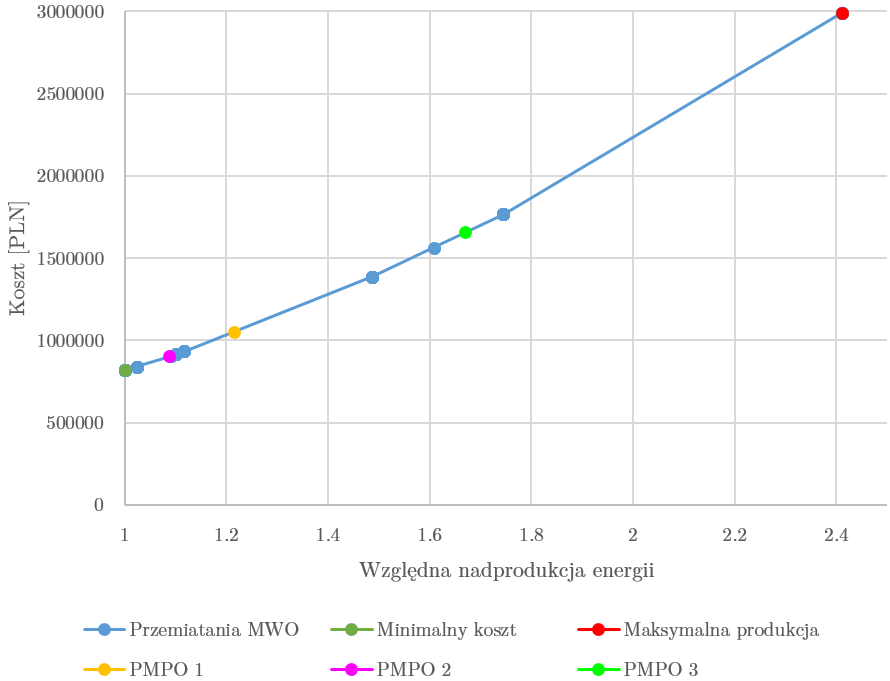
\includegraphics[scale=0.4]{plot_new.png}
\caption{Przestrzeń rozwiązań efektywnych w przestrzeni względnej produkcji i kosztu}
\label{fig:plot}
\end{figure}

%\printbibliography

\end{document}
